\chapter{Empirical Data}

For a successful case study based research, it is critical to collect the right type of data. Guest(2013) quotes in his book “Given our working definition of qualitative research, you can begin to imagine the range of possible data types that qualitative research might generate”, he describes various types of qualitative data that could be collected. Hence keeping those tips in mind the empirical data for this case was collected. This chapter focuses on consolidating all the empirical data that was gathered at Volvo GTT. \\

Initially, the KPIs under study are listed along with their definitions. Then the Strategy of the business unit in focus is described. The next part contains the data from KPI owners, Directors and the Vice-president of PE-Sweden. Here the insights of all these employees about KPIs is presented. The last part details the survey which was propagated to all PE-Sweden employees.

\section{PE Sweden KPI´s}

The fulcrum point of the whole thesis are the PE-Sweden KPIs. For this study, the KPIs used for financial year 2018 has been considered. In this section, the list of KPIs is presented with the area and the value in the figure \ref{fig:5.1}. Later the definition of each KPI is written.\\
Some definitions are directly taken from the internal website, whereas some of them have been defined based on the study by research students and inputs from the KPI owners.\\

\subsection{KPIs on Customer success}
\begin{itemize}
    \item \textbf{QJ lead time:} QJ refers to “Quality Journal”. It is the report used to manage the field quality solving process. This KPI directly relates to the value of customer success, as it is important that any field issues are solved soon.\\ 


     \item \textbf{New to Market ready (no. of open days):}
    This KPI refers to the time taken from a QJ is opened until it is completely solved and the product/system is ready to be used in market again. This process has multiple steps which may involve some changes in production and requiring complete testing again \\

     \item \textbf{New to containment action (no. of open days):}
    This KPI refers to the time taken since a QJ is opened and the problem is contained. This provides relief for the customer from the problem. This is different from the first one, as tested solution is not employed in the original product for all other customers.\\
    
    \begin{figure}[H]
    \centering
    \captionsetup{justification=centering, margin=2cm}
    \vspace{1cm}
    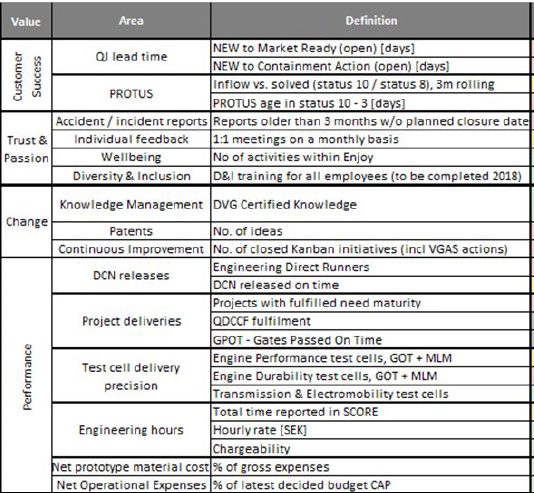
\includegraphics[width=14cm, height=12cm]{figure/auxiliary/fig51.PNG}
    \caption{ PE Sweden KPI List}
    \label{fig:5.1}
\end{figure}


     \item \textbf{PROTUS:}
    PROTUS is an acronym for PROTotype follow-Up System. PROTUS is a vital tool that allows to specify a test prototype, support the building of the prototype and to report assembly problems or deviations, support the testing of the prototype and to report problems linked with the production process (Volvo teamplace,2019)\\

     \item \textbf{Inflow vs solved (Status 10 / status 8), 3month rolling:}
    This KPI measures the ratio of incoming and solved PROTUS issues with 3 month rolling time. Status 10 refers when the PROTUS report is drafted and distributed. Status 8 is when the issue is completely solved. Overall, this KPI presents the whole picture of PROTUS process.\\

     \item \textbf{PROTUS age in status 10-3 (No. of days):}
    This KPI measures the time taken in days for a PROTUS report since it is distributed, reaches the responsible design department and the root cause analysis has begun. This KPI focuses on the initial process of PROTUS handling.\\
\end{itemize}

\subsection{KPIs on Trust and Passion}
\begin{itemize}
     \item \textbf{Accident/Incident reports:}
    This KPI keeps tab on the number of accident reports. The number of reports older than 3 months without planned closure date are listed..\\

     \item \textbf{Individual feedback:}
    This KPI measures whether the monthly 1:1 meetings are done by a manager with his/her team members. This was to ensure sufficient communication and personal development.\\

     \item \textbf{Wellbeing:}
    This KPI measures the number of activities done within the “Enjoy” program. This is to build employee engagement and help employees to build better relationships.\\

     \item \textbf{Diversity & Inclusion:}
    This KPI measured the number of employees who participated in the D&I training delivered by the company. The aim was to increase the awareness of employees regarding D&I in this new era of globalization.\\
\end{itemize}

\subsection{KPIs on Change}
\begin{itemize}
    \item \textbf{Knowledge management:} This KPI keeps tab on the number of employees completing DVG training. Design & verification guidelines (DVG) is a tool used in powertrain which supports knowledge management.\\ 

    \item \textbf{Patents:}
    This KPI counts the number of ideas developed to apply for a patent. It does not indicate the number of patents actually awarded, as it takes a long time.\\

     \item \textbf{Continuous improvement:}
    This KPI measures the continuous improvement activities/ideas by counting the number of closed Kanban initiatives. Basically, ideas provided by employees to improve a process/product was verified by a team of experts and feasible ideas were converted into Kanban initiatives.\\
\end{itemize}


\subsection{KPIs on Performance}

\begin{itemize}

     \item \textbf{DCN Releases:}
    DCN refers to Design Change Notice.The DCN is used to approve and publish changes in the product documentation (in KOLA). After approval, the DCN is an order to start up production preparation, purchasing and other downstream activities. (Volvo teamplace,2019)

     \item \textbf{Engineering direct runners:}
    This KPI is defined as the percentage of new parts which are not changed within 12 months Basically, it signifies how good the design was and the efficiency of product portfolio development process.

     \item \textbf{ DCN released on time:}
    This is relatively a simple KPI which measures the delivery precision. It is the ratio of number of DCNs released on time by the total number of DCNs released.

     \item \textbf{Project Deliveries:}
    The KPIs under this area measure the progress and effectiveness of projects. As visible from the table, it has 3 KPIs.

     \item \textbf{Projects with fulfilled need maturity:}
  It is defined as the number of projects which prove maturity at a given gate at prerequisite and/or attribute level. Maturity here means the ratio of agreed requirements regarding the product under development. It is a tricky KPI to define and objectively measure.

     \item \textbf{QDCF fulfilment:}
    QDCF is acronym for Quality, Delivery, Cost and Feature. Quality refers to project quality, delivery indicates delivery precision, cost is both project and product cost and feature is a customer expectation. The KPI is measured by the percentage of projects which fulfil all the QDCF criteria among the overall projects.

     \item \textbf{Gates passed on time (GPOT):}
    This KPI measures the flow of projects, with the aim to reduce R&D cost. It is defined as the percentage of gates opened out of the total number of gates scheduled during the month.

     \item \textbf{Test cell delivery precision:}
    All the three KPIs under this area measure the utilization of the test cells. There are three kinds of test cells namely, Performance, durability & electromobility. The KPI is measured as the ratio of actual/planned tests. But also the utilization of each test cell is also mentioned.\\
\end{itemize}


\subsection{Financial KPIs}
All the KPI´s listed below are hereby referred together as financial KPI´s as the main focus is on the cost.\\
\begin{itemize}
    
     \item \textbf{Engineering Hours:} This area has 3 KPIs under it. They are described below 

     \item \textbf{Total time reported in SCORE:}
This KPI measures the total project working time which is reported by employees in the IT tool SCORE. In simple terms it indicates time reporting.

     \item \textbf{Hourly rate:}
It is calculated by dividing the OPEX (operating expense) cost by total billable man hours with 6 months rolling. The usual OPEX costs such as employee salaries, consumables, fuel etc. is considered.  

     \item \textbf{Chargeability:}
It is measured as the ratio of billable hours/total available hours. It simply defines the amount of time spent on working on actual projects. 

     \item \textbf{Net prototype material cost \% of gross expenses:\\
Net operational expenses \% of latest decided budget CAP: }
Both these KPI describe themselves. These KPI´s are used by top management and finance department to calculate the cost deviations.\\

\end{itemize}


\section{Volvo GTT Strategy} 

The strategic priorities of the mother department leads the way for objectives and then KPIs for the teams under its umbrella. As PE-Sweden comes under GTT, the goals are translated from the strategic priorities. The 5 strategic priorities are presented in the figure \ref{fig:5.2} and then the major objectives are discussed.\\
    \begin{figure}[H]
    \centering
    \captionsetup{justification=centering, margin=2cm}
    \vspace{1cm}
    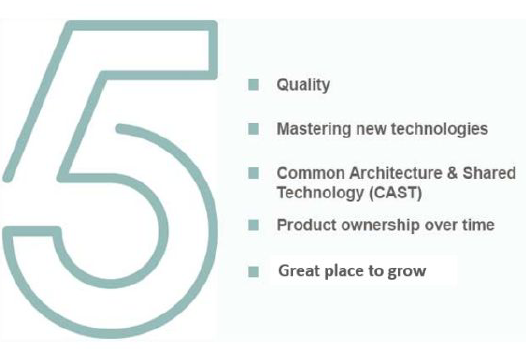
\includegraphics[width=13cm, height=8cm]{figure/auxiliary/fig52.PNG}
    \caption{5 Strategic goals of Volvo GTT}
    \label{fig:5.2}
\end{figure}
\begin{itemize}
    
     \item \textbf{Quality:} The main aim is to produce best quality products for the end customer in the market. The important objectives here are:
- Stable pre production drawing releases
- Improved ways of working with PROTUS (fault reporting system)
- Improved software and data quality
- Product oriented quality action group.

     \item \textbf{Mastering new technologies:}
To reach product leadership for all the brands within their competitive sets there is a need to master well-known as well as new technology. The plans are.
- An organizational model, ways of working, processes and governance for major new technologies
- New partnerships giving access to new technologies, input to more agile ways of working and speed up the work on existing technologies.

     \item \textbf{CAST (Common architecture and shared technology):}
Focus going forward: scalable affordable EE architecture allowing for rapid development of new functionality. Some of the most important goals are:
- Optimized modular architecture prepared for new technologies 
- Full implementation of Agile and Lean
- Scalable and affordable to roll out in steps.

     \item \textbf{Product ownership over time:}
To reach product leadership and increase customer satisfaction a clear product ownership over time should be established. This includes:
- Appointing product owners for components and systems as well as for services, features and complete vehicles 
- Clear product owner accountability for product evolution through the complete life cycle
- Chosen product owners with the business understanding, product knowledge, skills and means to secure product leadership, acting cross-functionally with the end customer in mind.

     \item \textbf{Great place to grow:}
GTT is regarded as the most sought after employer for both freshly graduated and experienced talents in selected competence areas. The objectives are:
- Proactive work with employer branding & attractiveness to secure employee retention and a steady supply of talents
- In-depth product, customer and automotive industry knowledge among Volvo employees
\\

\end{itemize}

\section{Data from KPI Owners}

It is important to have a clear picture on precise definition of each KPI, how they are being measured, how are the employees perceiving the KPIs and the top management's interest in each KPI. Hence, to gain this knowledge, the documents on the website were studied in the second phase of thesis and in the third phase the KPI owners were interviewed. The positives, drawbacks, issues and the suggestions mentioned by the KPI owners for each KPI have been consolidated in the section below based on the Values.

\subsection{Value-Customer success} There are 2 areas of KPIs under this value. They are QJ lead time and PROTUS.

\begin{itemize}
    
     \item \textbf{QJ lead time:} This area has 2 different KPIs, which measures the number of days from the start of the QJ till market ready and containment actions.They are as follows:
     NEW to Market ready and NEW to containment action
\\

As mentioned by the interviewees, the positive factor about this KPI was that it is being used by various teams to make improvement actions.
The drawbacks were, firstly, it measured only the number of days, but the magnitude of the QJ problem was not considered. To improve this the owners suggest to focus on speed of solving the QJ. Another drawback mentioned by KPI owner is the KPI needs to focus on measuring the performance and if the customer is satisfied with the solutions. The field failure frequency(FFF) also needed to be considered.\\

Apart from these issues, the problem with measuring this KPI was that the process and IT tools  were complex and the focus from all the engineers in all departments to work on QJs was necessary.
Suggestions on how the KPI could be improved was also given the interview which is to alter the focus area frequently, in order to concentrate on the various issues in each phase.

\item \textbf{PROTUS:} This area has 2 KPIs which are as follows::
     Inflow vs. solved (Status 10/status 8), 3 month rolling and
PROTUS Age in status 10-3.\\

The interviewees quote the following Positives, drawbacks and suggestions for improvement in regard to this KPI:\\

Positives:The data regarding this KPI is being updated on a daily basis, and is being followed by the top management. It is also used by the teams to make improvements. 
Drawbacks: This KPI has a complex  process to collect data, also there was no clear accountability of PROTUS.The focus of the present KPI is on the time, instead of the quality of solution. Also, updation of the KPI needed to be done on a regular basis. 
Suggestions: The major suggestion for improving this KPI was to reconsider measuring Inflow vs. solved PROTUS and the efficiency of solving them.

\end{itemize}

\subsection{Value-Trust and Passion}
This value includes 4 different KPIs as mentioned below:\\
Accident/Incident report reports, Individual feedback, Wellbeing and Diversity and Inclusion:\\

The inputs regarding these KPIs in general were that they could be measured or handled by supporting departments, instead of the engineers in PE. 
Interviewees mention that the KPIs like Wellbeing, individual feedback were needed previously to develop a culture, but now they are obsolete. Hence, such KPIs could be deleted or could be handled by other departments which focus more on work environment.

\subsection{Value-Change}
There are 3 KPIs under this value. The opinions of KPI owner is described one by one in detail.

\begin{itemize}
    
     \item \textbf{Knowledge Management:} The KPI for this area is measuring the “DVG Certified knowledge”.
A good thing the KPI owner mentions about this KPI is that it has high focus from the top management as it is the only way to build and reuse the knowledge in teams and it is also a part of global KPIs.
During the interview the owner pointed out a drawback about this KPI that it is difficult to measure and quantify the knowledge in general. There is a system for DVG certification and collection of that data, but that is not the only knowledge.
To improve those drawbacks interviewee also provides a suggestion that the new reorganization is in place, the new agile way of working might change the way knowledge is being measured based on the cycles of working. Hence this KPI needs to be adapted accordingly and redefined.

\item \textbf{Patents:} This KPI measures the “number of ideas” per month.The owner says that it is a good measure as it indicates the amount of innovation done or the ideas generated in the organization.

\item \textbf{Continuous Improvement:} As per the definition this KPI measures the “number of closed Kanban initiatives (including VGAS actions)”
The positive aspect of this KPI was mentioned that every employee is interested in continuous improvement, they strive to make improvements on a daily basis. Hence the objective behind the KPI to measure CI is good. But the drawback stated was that number of Kanbans is not the right measure, though it is being removed now.
\\
\end{itemize}

\subsection{Value-Performance}
This value contains 4 areas of KPIs. They are DCN Releases, Project deliveries, Test cell delivery precision and all financial KPIs.
The thoughts of KPI owners on each area of KPIs are discussed below.

\begin{itemize}
    
     \item \textbf{DCN Releases:} This Area measure 2 KPIs which are Engineering direct runners (EDR) and DCN released on time
\\

Engineering Direct runners is a KPI which indicates design effectiveness and efficiency. But there are a few drawbacks to this KPI. As stated by the interviewee this KPI belonged to a certain department, but was being handled by someone else. The major drawback of this KPI is that it is not helpful to drive or change behavior Hence driving a wrong behaviour, says the owner. Due to lack of top management interest in this KPI, it is not being utilized efficiently. Root cause analysis in case of bad result is not done to fix the issues.
In order to improve this KPI, the owner says that iit needs to be handled by the right department. Also, conducting pulse queries and updates would be more effective than monthly updates.\\

DCN released on time is another KPI which is simple to measure. The interviewee states a few issues with this KPI, which are, firstly it drives the wrong behaviour in teams. Secondly, the agreed completion date is not lined to the project progress. Lastly, no periodic review or learning in the team happens related to DCN releases.
To improve this the suggestion given was “to communicate with the PMEs for exact required date of release and ensure the KPI reflects the reasons for delay i.e the K-DCN cases.”\\


\item \textbf{Project deliveries:} Project deliveries are being measured with the help of 3 different KPIs which are as follows:
Projects with fulfilled need maturity, QDCF fulfilment and
GPOT- Gates passed on time
\\

The first KPI indicates the maturity of projects with respect to gates. The owner of this KPI provides the description that, when a project is initiated, certain number of prerequisites are mentioned, and the main design requirements are connected to the gates. Hence, the ratio of agreed requirements to the total requirements is the maturity of the project. A positive about this KPI is that it is discussed with the steering committee. But drawback of this KPI, as mentioned by the interviewee was that the definition of this KPI was abstract, making it difficult for others to understand the aim of the KPI. Another drawback is that, the values are technical and hence hard to understand. The value could also be misleading in case the requirements are not agreed.\\

The second KPI was “QDCF fulfilment”
The owner provides the following positives and drawbacks on this KPI as follows:
Positives: It is a widely established KPI.
Drawbacks: It has a very complicated to measure and it is seldom updated in a year. Major drawback with this KPI is that, in order to fulfil the deadlines it creates a wrong behaviour in employees.\\

The third KPI is the Gates Passed on Time(GPOT), which measures the delivery rate of the projects which had drawback as quoted by the owner. This KPI is very subjective in nature, which does not consider the project size and complexity. It drives the wrong behaviour in the employees, as the PROTUS are closed in order to pass the gate, in turn reducing the quality of the work. The progress of work, between the gates is missed out.
The suggestion given by the interviewee to improve this KPI was to reconsider by keeping the progress of the project in mind.\\


\item \textbf{Test cell delivery precision:} This area is measured with 3 different KPIs, which are as follows: Engine performance test cells, Engine durability test cells and Transmission and Electromobility test cells. All the 3 KPIs measure the resource utilization, and the following drawbacks suggestions were stated by the owner during the interview:\\

Drawbacks: The departments handling the testing, do not know if it the right test that is being conducted, which is not reflected in the KPI. These KPIs also do not depict the quality of the tests conducted, which is more important, than the utilization of the test cells. 
Based on similar requirements the following suggestions were given for improvement of these KPIs
Suggestions: Factors like utilization of the test data, the quality of the test results need to be considered. The focus needs to be given on delivery precision of  the test cells. 
The efficiency of planning and prioritizations methods need to be increased and proactive testing needs to be given a thought in order to find faults.
\\

\item \textbf{Financial KPIs:} 

There is a set of 5 KPIs under the financial KPIs. There were general comments on each of these KPIs were given during the interviewees as follows:\\

Total time reported in SCORE - This KPI is not truly owned. The purpose of this KPI was to make the employees report time. 
It is not needed to be measured anymore as it becomes a routine, hence can be removed as a KPI.\\

Hourly rate [SEK] - This KPI is a quick indicator can be used to depict the engineering hours. But it it not efficiently utilized. But it merges the working hours and cost into one measure. Some values of the KPI are crossing 100 percent which signifies there may be some improvements needed in definition.\\

Chargeability - The owner mentions that this KPI drives  wrong behaviour and hence can be deleted. In context of Sweden not so useful as people are more honest in time reporting. Often not a true figure of reality.\\

Percentage of gross expenses - It focuses mainly on the material cost, hence it can be improved such that based on the phase of the projects in PE ,the gross expenses can be kept track of.
Also longer stretches like 3 months rolling can be used for such KPI.\\

Percentage of latest decided budget CAP - This is a good KPI and could be retained.\\

Concluding these views, the following picture was made figure \ref{fig:5.3}. Where the red depicts the KPIs that must be removed, the green represents the KPIs that could be kept as they are and the yellow are the KPIs that could be improved.\\
\end{itemize}
    \begin{figure}[H]
    \centering
    \captionsetup{justification=centering, margin=2cm}
    \vspace{1cm}
    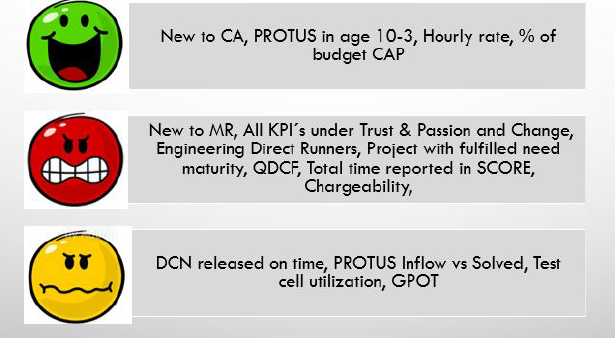
\includegraphics[width=15cm, height=9cm]{figure/auxiliary/fig53.PNG}
    \caption{ KPIs categorized based on interview inputs}
    \label{fig:5.3}
\end{figure}

\section{Data from Directors and VP Interview}

After the interviews of KPI Owners, it was important to know the intuition of the Directors who lead the 7 departments at PE-Sweden. As these directors are responsible to guide the engineers towards strategically urgent tasks, take decisions based on monthly KPI figures and provide the necessary support to resources. The top management perspective on KPI usage at PE -Sweden was prominent in order to understand the KPI governance structure.\\

Directors of PE-Sweden act as a link between the top management and the engineers. Their tasks include, monitoring the progress of projects in their department, analysing the monthly KPI figures in management meetings, monitor the performance etc. The main intention of these interviews was to know their way of working, insights on KPIs, strategy, performance measurement and future needs. The questions were formulated keeping in mind the following dimensions as seen in the figure \ref{fig:5.4}. The X-axis represents the time period, whether the intention was to gather information about the present or the future. Y-axis indicates the aspect whether the question was more on day to day operative side or on the broad strategic side. The idea behind each question and the combined insights are presented individually.
    \begin{figure}[H]
    \centering
    \captionsetup{justification=centering, margin=2cm}
    \vspace{1cm}
    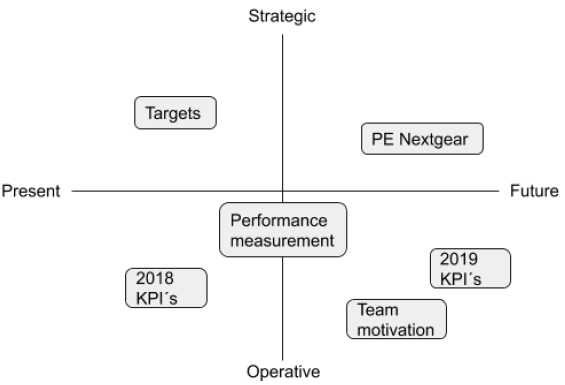
\includegraphics[width=12cm, height=9cm]{figure/auxiliary/fig54.PNG}
    \caption{ Discussion topics with directors}
    \label{fig:5.4}
\end{figure}

\begin{enumerate}
    \item \textbf{How intensely do you follow the PE-Sweden KPIs?}\\
    
    The intent here is to understand how the present KPIs elicited the behaviour of directors and their individual way of dealing with these KPIs. The answers provided by all the directors are coded and the key words are described here. To respect the privacy of the individuals, the insights are combined and presented.\\
    
    \textbf{Keywords} Do not follow KPIs much, Do not follow KPIs at all, Focus on some important KPIs\\
    
    The PE-Sweden KPIs as such did not provide much value to the directors. Some of them followed it monthly to check the numbers, some focussed on the most important KPIs which mattered to their daily work and almost everyone agreed that each of the 23 KPIs did not provide much value to focus their attention on them. Overall, there was clearly a lack of intent to follow up and work with these KPIs.\\
    
    This lack of intent was created due to these prominent reasons:
Too many KPIs, some KPIs do not drive the right behaviour, less visibility of KPIs down the line, unclear objective behind some KPIs. These reasons coupled together with other factors made them to not work intensively with the present 2018 PE-Sweden KPIs.\\

\item \textbf{Views about present PE-Sweden KPIs.}\\

The directors were asked to comment on individual KPIs to get their views on them. The purpose here was to know what they felt about the KPIs at the first moment. The answers are more general and do not delve into the technicalities of each measure. In addition to whether they thought the KPI was good/bad, additional comments on the problem area and solutions were elicited. Table \ref{tab:Inputs} displays with keywords gathered by coding the interviews and discussed in brief detail later.\\


\textbf{QJ lead time} 
All the directors thought that this is one of the most important KPI which is discussed in meetings. The specific KPI of “New to Containment action” was preferred as compared to “New to Market ready”. But almost all of them agreed that a new way of defining customer success using QJs is needed. They felt the present way of measuring QJ lead time does not consider the magnitude of the problem at hand. Also, as the process of solving issues has many steps the focus area need to be defined. Based on the focus area the solutions can be developed on which each department can contribute. One of the clear suggestion was to concentrate on duration of First known failure till the corrective action which perfectly describes the transition from unhappy to happy customers.\\

\textbf{PROTUS} Along with QJ lead time, PROTUS is one of the most important KPI which cuts across almost all departments. The protus data sheet is updated daily and any employee can view the progress of each issue. The directors seem to be divided on the favour of one of 2 specific KPIs. Some prefer “Inflow vs solved” should be focussed as it presents the whole picture. Whereas, some prefer “Protus age 10-3” would give better focus. But the terms of agreement among all directors are the speed of solving PROTUS issues should be important rather than the number of PROTUS and the present communication/discussion in meetings is very good which reiterates the importance of this KPI.\\

\textbf{Accident/Incident reports} This measure indicates the safety of employees. PE-Sweden comprising mostly product development engineers, many feel this KPI does not take much importance. However, in testing department this KPI does matter as there is risk of injuries. The directors agree that although the safety of employees is paramount and steps are taken to ensure no accidents, this should not be measured as a KPI. Accident reports can be just informed to top management and published monthly in website, but no need to keep this as KPI.\\

\begin{table}[H]
    \centering
    \captionsetup{justification=centering, margin=2cm}
    \label{storage}
    %\scalebox{0.5}{%
    \begin{tabular}{|p{4cm}|p{10cm}|c|} \hline
    \textbf{KPIs} & \textbf{Keywords described}\\
    \hline
     QJ lead time \vfill \hfill& Very important, not good results, badly measured, define focus area, focus on the magnitude of problem, focus on unhappy to happy customers\\\hline
     PROTUS & Spontaneously followed, good, focus on the whole process, focus on stage 10-3, dynamic KPI, speed is important \vfill \hfill\\\hline
     Accident/Incident reports & Legal requirement, important, just present in list, not meaningful as a KPI\\\hline
     Individual feedback 1:1 meetings & Not good as a KPI, depends on individual, obsolete with new way of working \\\hline
     Well being & Not good as a KPI, events are more important, drives good behaviour \\\hline
     Diversity and Inclusion & Not good as a KPI, no need, not valid, more of how you act\\\hline
     Knowledge & Is it really needed as KPI?, not sure what it gives , need to rethink way \\\hline
     Management & of defining it \\\hline
     Patents & Good measure, indicates innovation \\\hline
     Continuous improvement & Debatable definition, need to redefine, scrap it \\\hline
     DCN releases & Okay KPI, reduce late DCN, rethink how the numbers are perceived, matters a lot, Good KPI, need to rework \\\hline
     Project Deliveries & NGood, well established, fairly okay, complicated, possibility of manipulation, too many of them, need only one KPI \\\hline
     Test cell delivery precision & Measures only utilization of resources, quality of testing is not measured, not good, concentrate on activities after test\\\hline
     Financial KPI´s & Reduce the number of financial KPIs, not discussed or reviewed\\\hline
    \end{tabular}%}
    \caption{Inputs from Directors on each KPI}
   \label{tab:Inputs}
\end{table}\\

\textbf{Individual feedback} This measures the 1:1 monthly meetings. Every director feels that this should not be a KPI, but rather infused as a company culture. The new setup of being more Agile automatically brings in more communication making the 1:1 meetings obsolete. As the engineers work on a variety of tasks, the frequency of meetings is more situational and dependent on the job profile. Overall, everyone agrees to scrap it as a KPI.\\

\textbf{Wellbeing} This is measured by the number of activities within Enjoy. Almost every director opines that is should not be a KPI. Although, it drives good employee behaviour everyone feels that the quality/theme of events is more important than to count the number of events. It is one of the KPIs which is overlooked in the list.\\

\textbf{Diversity & Inclusion} A training was given to employees regarding the topic during 2018. Every director feels that this should not be used as a KPI. They feel that diversity & inclusion is more about behaviour and awareness.\\

\textbf{Knowledge management} Similar to diversity & inclusion, a training is given and measured to visualize this KPI. Although the aspect of knowledge management is very important for any firm, the way of defining plays a prominent role. Some directors notice that the KPI in present form does not clearly say what value it provides. Therefore, it needs to be rethought to define knowledge management and implement it to be a true learning organization. But, everyone agrees that this need not be a KPI, rather than an action plan or included in way of working.\\

\textbf{Patents} This KPI measures the number of patents filed. By definition, it clearly indicates the innovation happening in the firm and promotes idea generation. But, most directors were not clearly onboard to follow or scrap the KPI, but rather talked about it as a good measure and we need to keep it.\\

\textbf{Continuous Improvement}  Every organisation needs to focus on continuous improvement. Here in PE-Sweden, improvement ideas are presented which are then evaluated after translating them into Kanban initiatives. It is not entirely clear for all the directors. Many of them feel to redefine the KPI to make it more effective. Some directors who are more connected to this KPI, inform that it has been scrapped for usage in future.\\

\textbf{Engineering direct runners}Almost every director identify it as a “Ok” KPI. Directors who work with more detail on this topic opine that there needs to be more loops in early phase of DCNs to reduce chances of late changes. But everyone subtly agree that some improvements are definitely possible.\\

\textbf{DCN released on time} Directors agree that a DCN released on time matters a lot. The KPI also sounds good with respect to how it is defined in a simple manner. Most directors discern that it is a good KPI and need to be kept. But, some directors who work more hands on feel it should be slightly modified to drive right behaviour. One suggestion was to perform FMEA on DCNs to improve.\\

\textbf{Project Deliveries} The project deliveries are represented by 3 different KPI´s. Almost all the directors feel that they are too many and create confusion. Everyone agrees to reduce the number of KPIs measuring project delivery to only one. The views on the two important KPI´s are described below.\\

\textbf{QDCF fulfilment} The opinions are divided about this KPI. Some directors feel that it is well established and okay to use. Whereas, directors keenly working on QDCF opine that it is too complicated to propagate the true intention and evaluation. Also, it does not add much value to the notion of project deliveries and hence can be scrapped.\\

\textbf{GPOT} Most of the directors feel that this KPI is fairly okay. It is not complicated as QDCCF. But, there is a possibility of rushing some tasks to achieve the target thus driving wrong behaviour. Integrity of leaders plays an important part in order to trust the numbers. The directors agree that this could be the one KPI defining project deliveries with some modifications.\\

\textbf{Test cell delivery precision} As mentioned in previous sections, this section is made up of 3 KPIs which measure the utilization of the test cells. Every director agrees that the quality of tests should be of primary focus and not the number of hours. The present KPIs does not provide much value rather than presenting resource utilization. Director responsible for this KPI opined that the actual need of the tests, how the test reports are used after the testing should also be considered. Overall, the directors feel that the present test cell KPIs are not good and need to be redefined with quality of testing as cornerstone.\\

\textbf{Financial KPIs} Most of the directors had no specific comments to make on the 5 financial KPI´s. They felt that it is not their forte to look and contribute for it, rather than just view the numbers once in a while. Some directors observed to reduce the number from 5 to 2 and expressed discontent with some KPIs such as total time reported in SCORE. One of the suggestions was to use Chargeability KPI and forego the other 2 engineering hours KPI´s. Overall, these were of not much interest to directors to comment on.\\

\item \textbf{How the company goals are allocated to you?}
The main intention was to gather how directors receive the strategic goals, yearly objectives or quarterly targets. As reflected in the fig, this lies in the quadrant of strategic and present. Intentionally, the question was not too specific so as to elicit broad range of answers according to their perception.\\

\textbf{Keywords} Top management meeting, soft targets, discussion, dialogue.\\

The company goals were communicated and discussed with all the directors during extended top management meeting. The directors clearly mentioned how the goals were allocated to them previously and now. Previously, there was much more hard targets presented to them with strict deployment of business strategy. It provided much focus for the task at hand. But now, there are more soft targets which are discussed during meetings. This presents more flexibility to the directors to decide themselves about the course of action. Also, one factor to be noted is that the discussions during the directors and top management are frequent and often in the form of dialogues.\\

\item \textbf{How do you deploy the strategy to your department?}
This question acts as the next step for the previous question. After receiving or discussing the goals allocated to them, it was important to know how directors go ahead with deploying the targets to their respective departments.\\

\textbf{Keywords} Meetings and follow-up, set targets to team, action log, PI planning, break down goals and allocate task.\\

Each director had his/her unique way of deploying the strategy. Some directors preferred to further breakdown the goals into targets and follow them with weekly meetings or action logs. Some directors preferred to have more constant communication with their teams and be updated about the proceedings. The intention was to realize the goals rather than focusing on the way of working. But every director was eager to work systematically in this regard and have an improved approach.\\

\item \textbf{How do you measure the performance of your teams?}
Performance measurement aspect plays an important part for directors to visualize how far they have achieved their targets. The insights of PE-Sweden directors are discussed below.\\

\textbf{Keywords} Drive team focus on deliverables, speed of achieving goals, PBT tool, ad-hoc, dialogues, concentrate on daily tasks.\\

As expected, there was different ways how directors went about measuring performance of their teams. Most of the directors concentrated on their meetings with various group managers, follow up of daily tasks and constant dialogues to be appraised about the teams performance. Some preferred to use PBP tool and follow up on the mentioned targets. Overall, the style followed by Directors was more ad-hoc and dependent on the functions of their department. But most of them felt the need to have a better IT tool where they could set up developmental plans and follow up on them periodically to have a clear idea about the set targets.\\

\item \textbf{How would you motivate your team to work with KPIs?}
This question is more into the future. As PE-Sweden was undergoing changes during Nov 2018 until April-2019, directors were unsure about the goals and KPIs. By answering this question, directors have described their plans to work with future KPIs in PE Nextgear.\\

\textbf{Keywords} Clear and right KPIs, be a role model, focus on daily tasks, visual communication of KPIs.\\

As there were too many KPIs with some unclear definitions, many directors felt a set of few precise KPIs would itself motivate and help them motivate their teams to work with them. Some directors pointed out the lack of visual communication regarding KPIs which is hindering the engineers to see them. Some directors opined the need to be a role model and inspire their teams to put effort on KPIs. Most of the directors prefer to concentrate on daily tasks through KPIs which will automatically bring in the acceptance and motivation for their teams.\\

\item \textbf{On what should future KPIs be built on?} This was the last question for the directors. After presenting their views on strategy, KPIs, performance measurement, this question provided them the opportunity to combine all their thoughts and inform us what do they want in the future KPIs.\\

\textbf{Keywords} few KPIs, measure the flow of tasks, focus on culture, trust, mindset and customer, drive right behaviour.\\

The needs for perfect KPIs could go on forever. But, the directors aptly presented their thoughts on future KPIs with some real life examples of work conditions and the way of working at Volvo. Everyone wanted to work with handful of KPIs focusing on the flow of daily tasks, in accordance with the Volvo culture, driving right employee behaviour and concentrating on product performance.\\

\end{enumerate}


\section{Contents of the survey}
Once the KPI owners and directors were interviewed, a top management perspective was understood. The next phase was to perceive the mindset of the employees or the teams. In one of the books, Robinson, S.(2012) mentions that to get successful pursuit of this performance improvement, it is necessary to have everyone on board, like the management, employees etc. Hence, to study what the employees think about the KPIs and their needs regarding the same, a survey was conducted.\\

The survey was the result of extensive academic research on various aspects such as Survey design, different stages of conducting survey, the analysis methods etc. which are described in the theory section. Inculcating all the factors mentioned in the academics, all the available scales of measurement such as Nominal, ordinal, multiple choice, open and close ended questions and Kano questionnaire were employed.\\


A pilot test was conducted with the product documentation team, based on the feedback and results improvements were before sending out to the target group. This survey was sent out to all the employees under PE sweden, which consisted of 7 different departments and around 800+ people in total. The target was to get responses from approximately 20\% of the target population, and this was successfully achieved \\

The survey was structured in a way that it could match the way interviews were conducted previously. It had 6 sections, which are described below:\\

\begin{itemize}
    \item The first section was framed to understand the demographics of the employee answering the survey. In order to keep the identity of the person anonymous, basic questions like their department and experience were asked.  
    \item The second section had an objective to find the employee's understanding of KPIs. What they think about KPIs, do they follow them etc 
    \item The next section focused on their broader understanding or awareness of the strategic goals. The 5 strategic goals were presented and their knowledge towards them was found.
    \item The fourth section was on their view about performance measurement. How do they measure if they are performing better and their thoughts about the performance management tool.
    \item Section five was designed and analyzed to find the needs of the employees. Based on the theoretical study and present conditions, the questions were made according to the  KANO framework. Major conditions covered in this section were Strategic cascading, Documentation, Buy-in from teams and visualization.
    \item The last section was open ended questions about the new organizational change and future KPIs.
\end{itemize}
Now the gathered empirical data will be described briefly section wise. The purpose of the questions in each section along with the graphs or qualitative short answers are presented. The detailed survey questionnaire has been attached as Appendix (2) in the end of the report for further reference.\\

\subsection{Demographics}
As the purpose of the survey was to just gather the insights of employees, more personal details were not needed. Only 2 kinds of demographic data was collected for the survey. The first one is the departments. It was important to know that there is sufficient representation from engineers belonging to all the 7 departments at PE-Sweden.As visible from the fig 5.5, The response rate varied between 8 - 23\%. 
%    \begin{figure}[H]
 %   \centering
 %   \captionsetup{justification=centering, margin=2cm}
 %   \vspace{1cm}
 %   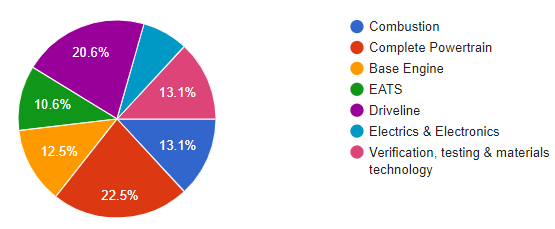
\includegraphics[width=10cm, height=6cm]{figure/auxiliary/fig55a.PNG}
 %   \caption{ Demographics results from survey}
 %   \label{fig:5.5a}
%\end{figure}
 %   \begin{figure}[H]
%    \centering
%    \captionsetup{justification=centering, margin=2cm}
%    \vspace{1cm}
 %   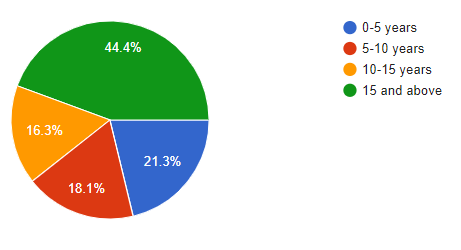
\includegraphics[width=10cm, height=6cm]{figure/auxiliary/fig55b.PNG}
%    \caption{  Demographics results from survey}
%    \label{fig:5.5b}
%\end{figure}

\begin{figure}[H]
  \centering
  \begin{minipage}[b]{0.5\textwidth}
    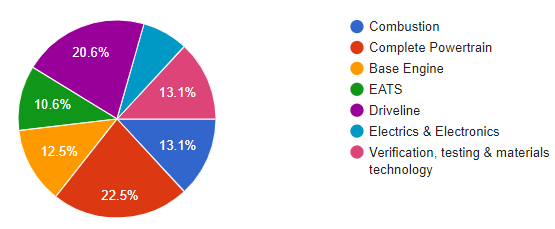
\includegraphics[width=\textwidth]{figure/auxiliary/fig55a.PNG}
    \caption{Demographics results from survey}
    \label{fig:5.5a}
  \end{minipage}
  \hfill
  \begin{minipage}[b]{0.4\textwidth}
    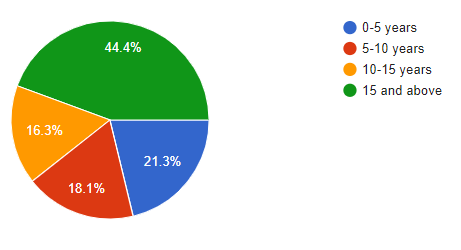
\includegraphics[width=\textwidth]{figure/auxiliary/fig55b.PNG}
    \caption{Demographics results from survey}
    \label{fig:5.5b}
  \end{minipage}
\end{figure}
The second demographic data was about the experience of employees. Idea was to receive responses from new employees as well as experienced Volvo veterans to gather various perspectives. The final data showed an impressive 44\% responses from employees with >15 years of experience. The second highest response rate was from the newbees with 0-5 years experience presenting their thoughts as well. Overall, the responses covered the whole spectrum fulfilling our intention\\

\subsection{About KPI´s in general}
It was essential to understand how employees perceive KPIs. Unless the understanding and the feelings from employees are not understood, any steps taken to improve KPIs would not bear fruit. This section presented them with simple but thoughtful questions eliciting their interpretation of KPIs. Most of the questions were multiple choice or yes/no type, along with option to write their own answer as well. \\

\begin{enumerate}
    \item \textbf{“What do you feel about KPI´s in general?}\\
     As shown in Fig \ref{fig:5.6} the majority of the response was that it is a top management thing. Only around 30 employees believed that it was their progress chart as well. 13\% of them informed they did not have any idea about the significance of PE-Sweden KPIs.
    \begin{figure}[H]
    \centering
    \captionsetup{justification=centering, margin=2cm}
    \vspace{1cm}
    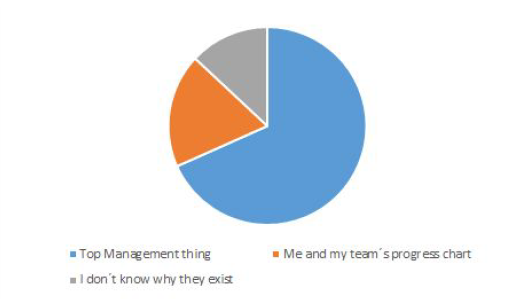
\includegraphics[width=12cm, height=7.5cm]{figure/auxiliary/fig56.PNG}
    \caption{What do employees feel about KPI in general?}
    \label{fig:5.6}
\end{figure}
    \item The second question probed the frequency of using KPI´s in day to day work and meetings. 60\% respondents mentioned that they sometimes discussed KPI´s in their teams with 37\% mentioning they never do it. Only a minority of employees informed that they often discuss the KPI´s with their teams.
    
\begin{figure}[H]
    \centering
    \captionsetup{justification=centering, margin=2cm}
    \vspace{1cm}
    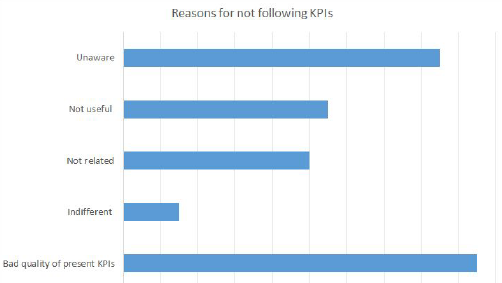
\includegraphics[width=12cm, height=7.5cm]{figure/auxiliary/fig57.PNG}
    \caption{Reasons for why employees did not follow the KPIs according to survey}
    \label{fig:5.7}
\end{figure}
    \item The third question was to know if they followed the KPI´s or no. Around 70\% majority voted that they do not follow the KPI´s with the reasons to do so. The reasons mentioned are coded into various groups and presented briefly in the figure \ref{fig:5.7}\\
The reasons were coded in various categories, out of which 5 major categories are represented in the graph above. Each of the category has been described below:\\

\begin{enumerate}
    \item \textbf{Unaware:} This group has second largest count. The people under this group are not aware either about KPIs or where to find them.\\
    \item \textbf{Not useful:} The respondants under this group have an opinions that KPIs are not an efficient method or tool to measure performance. This view is not specific to Volvo KPI, but it is generally about using KPI as a tool. This also includes people who thought they did not have time to use or look at the KPIs.\\
    \item \textbf{Not related:} This set of responses consists people who think their work cannot be measured, or the KPIs are not related to their work at all.\\
    \item \textbf{Indifferent:} The respondents under this category were indifferent about using the KPIs, they followed them if shown in the meetings, but did not follow the KPIs personally to manage tasks or meet target \\
    \item \textbf{Bad quality of present KPIs:} The last group of people showed interest in the present KPIs, they did not follow them due to the quality of the present KPIs. Various suggestions on how they could be reconsidered were mentioned such that it could satisfy their needs, or make them feel motivated to use the KPIs. \\
\end{enumerate}

    \item The last question in this section was to know which KPI´s are important and are mostly followed by employees. Option was given to choose multiple KPI´s which they work on. Based on the responses received the top 5 most followed KPI´s are as follows. PROTUS, Project Deliveries, QJ lead time, DCN Releases, Test cell performance.\\
\end{enumerate}

Therefore, the data gathered in this section clearly presents the general sentiment of employees regarding KPIs and further helps in suggesting future improvements.\\

\subsection{Strategy}
For the success of any business strategy, it is important that it penetrates at all employee levels. The intention in this section is to know the level of awareness among employees about the strategic goals of GTT, value of the present communication channels used to broadcast the strategy and how the strategic goals are translated to targets for employees by their immediate manager.

\begin{enumerate}
    \item The first question checked the level of awareness of the strategy among Powertrain engineers. The Volvo GTT strategy was presented and employees voted their knowledge about them using 4 levels, 1 being the lowest and 4 being the highest. As visible in figure \ref{fig:5.8}, most employees felt that they were aware of the strategy as approximately 80\% settled with level 3 or 4 with 47\% mentioning that they were very well aware.
\begin{figure}[H]
    \centering
    \captionsetup{justification=centering, margin=2cm}
    \vspace{1cm}
    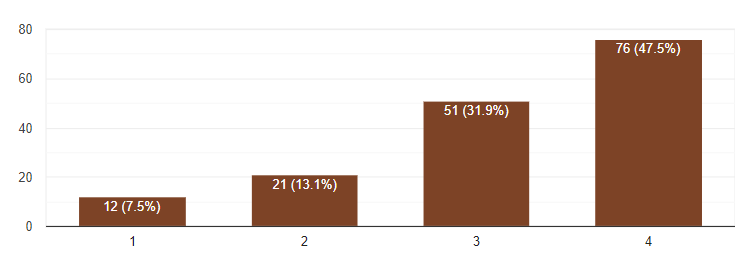
\includegraphics[width=12cm, height=6cm]{figure/auxiliary/fig58.PNG}
    \caption{How well were the employees aware about strategy}
    \label{fig:5.8}
\end{figure}    
    \item The second question was to quantify which communication methods were used by employees to read about the strategy. Again, this was a multiple choice question where they could choose from many options. The most popular tool was “Violin” the internal website of Volvo Group. Other options selected can be seen in the figure \ref{fig:5.9} 5.9 

\begin{figure}[H]
    \centering
    \captionsetup{justification=centering, margin=2cm}
    \vspace{1cm}
    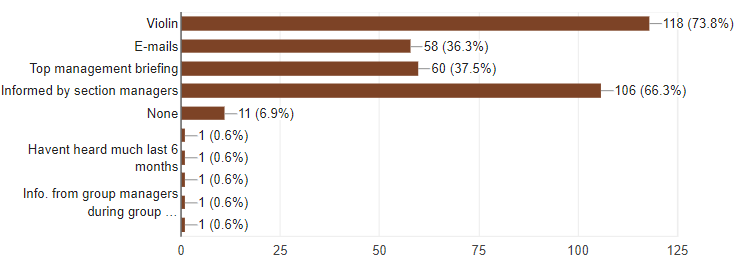
\includegraphics[width=14cm, height=6cm]{figure/auxiliary/fig59.PNG}
    \caption{ Communication ways used to propagate strategy}
    \label{fig:5.9}
\end{figure}

    \item The third question probed how their managers translated the higher level goals to them. This was a subjective answer where they could provide their insights briefly. The various replies are grouped together based on the similarities and the coded data is presented below in the figure \ref{fig:5.10}.\\
    \textbf{Keywords:}\\
    Unclear/No idea, Not done at all, In group meetings, Reorganization, Good. 
    The number of opinions for each of the keyword used is shown below. \\

\begin{figure}[H]
    \centering
    \captionsetup{justification=centering, margin=2cm}
    \vspace{1cm}
    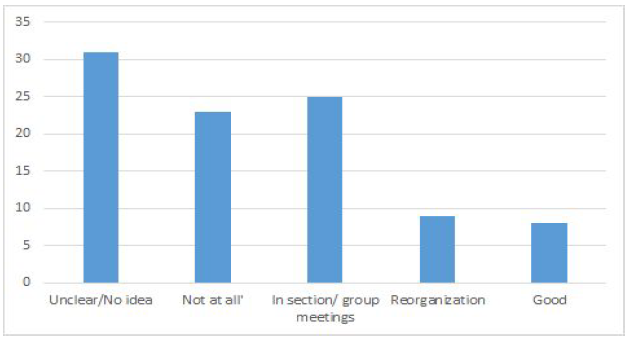
\includegraphics[width=12cm, height=7.5cm]{figure/auxiliary/fig510.PNG}
    \caption{ How are the goals translated to employees?}
    \label{fig:5.10}
\end{figure}
  
    \begin{enumerate}
    \item \textbf{Unclear/No idea:} Most of the people opined this. They were unclear about how the strategic goals are translated to them by their managers.\\
    \item \textbf{Not done at all:} Around 23 respondents clearly informed that the translating or cascading of goals was not done at all.\\
    \item \textbf{In section/group meetings:} Around 25 employees agreed that they discuss the top level goals during their meetings and gain the information from their managers.\\
    \item \textbf{Reorganization:} Some employees inferred that due to the reorganization this might be stopped or changed and hoped that they would receive the goals once it is complete.\\
    \item \textbf{Good:} Very few employees opined that their managers did a good job in translating the higher level goals to team targets.\\
\end{enumerate}
\end{enumerate}

\subsection{ Performance measurement}
This section was rather small with only 2 questions. The intention here was to gather how employees measured their performance and how the previous performance management tool aided them to achieve their targets.\\

The first question was a multiple choice probing “how do you know that you are performing well?”. The most preferred option was through feedback from manager/teammates, followed by I meet deadlines set for my team. This clearly reflects the impact of team meetings on the individuals. The various responses can be seen in the figure \ref{fig:5.11}
\begin{figure}[H]
    \centering
    \captionsetup{justification=centering, margin=2cm}
    \vspace{1cm}
    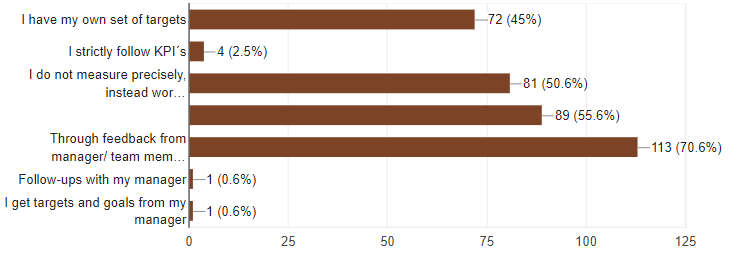
\includegraphics[width=15cm, height=6cm]{figure/auxiliary/fig511.PNG}
    \caption{How did the employees know they are performing well?}
    \label{fig:5.11}
\end{figure}

\begin{figure}[H]
    \centering
    \captionsetup{justification=centering, margin=2cm}
    \vspace{1cm}
    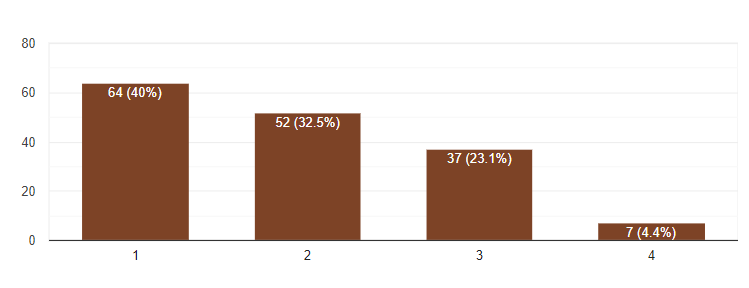
\includegraphics[width=15cm, height=6cm]{figure/auxiliary/fig512.PNG}
    \caption{Employee preference on PBP tool}
    \label{fig:5.12}
\end{figure}
The second question elicited the opinion of employees on previous performance measurement tool. They expressed how helpful was the tool by scoring 1-4, with 1 being the lowest and 4 being the highest. As visible from the figure \ref{fig:5.12}, around 70\% of responses were in the first half clearly mentioning that it was not so helpful.
\subsection{Future KPI´s}
This section was interesting because it elicited the needs of the employees. As mentioned before, this section focussed on 4 aspects, namely Strategic cascading, Documentation, Buy-in from teams and visualization. Kano questionnaire was used to get the needs of people without asking directly what they wanted.  \\

Based on the Kano theory mentioned before and the analysis method used. The following results can be obtained from the data.\\


\begin{enumerate}
    \item \textbf{Q1: How would you feel if strategic goals were/were not broken down and communicated to you ?}\\ 

The intention was to quantify and gather employees perception about the need for clear strategic cascading. As this was identified as an important area to increase the usefulness of KPIs.\\


 
 
\begin{table}[h]
    \centering
    \begin{tabular}{|c|c|c|}
    \hline
    \textbf{Need Characteristics} & \textbf{Number of responses} \\
    \hline
     Must be & 70\\\hline
     One dimensional & 30\\\hline
     Attractive & 11\\\hline
     Indifferent & 36 \\\hline
     Reverse & 4\\\hline
     Questionable & 9\\
    \hline
    \end{tabular}
    \caption{KANO analysis for Question 1}
 %   \label{tab:KANO1}
\end{table}


    \item \textbf{Q2: How would you feel if a document of objectives/targets is/is not shared with you by your Group Manager?}\\

The intention was to elicit if the documentation of the objectives was necessary for employees. As most of these targets are discussed during team meetings and not documented, some directors felt the need to have clear documentation to verify later and at same time increase the awareness among employees.\\

\begin{table}[h]
    \centering
    \begin{tabular}{|c|c|c|}
    \hline
    \textbf{Need Characteristics} & \textbf{Number of responses} \\
    \hline
     Must be & 52\\\hline
     One dimensional & 30\\\hline
     Attractive & 18\\\hline
     Indifferent & 47 \\\hline
     Reverse & 5\\\hline
     Questionable & 8\\
    \hline
    \end{tabular}
    \caption{KANO analysis for Question 2}
    \label{tab:KANO2}
\end{table}


    \item \textbf{Question 3: How would you feel if the KPI´s were/were not clearly defined and communicated visually?}\\

After the initial interviews with KPI owners and directors, there were some comments describing the vagueness of KPI´s and the aspect of KPI´s not being visible to most of employees. This question was asked what employees really wanted in this regard.\\

\begin{table}[h]
    \centering
    \begin{tabular}{|c|c|c|}
    \hline
    \textbf{Need Characteristics} & \textbf{Number of responses} \\
    \hline
     Must be & 39\\\hline
     One dimensional & 326\\\hline
     Attractive & 13\\\hline
     Indifferent & 71 \\\hline
     Reverse & 3\\\hline
     Questionable & 8\\
    \hline
    \end{tabular}
    \caption{KANO analysis for Question 3}
    \label{tab:KANO3}
\end{table}


    \item \textbf{Question 4: How would you feel if you could/could not contribute to develop and follow the KPI´s?}\\

Employee interest and contribution plays a paramount role in success/failure of any initiatives. Therefore, our idea was to understand how employees feel if they could contribute to work on the KPI´s rather than just following them.\\

\begin{table}[h]
    \centering
    \begin{tabular}{|c|c|c|}
    \hline
    \textbf{Need Characteristics} & \textbf{Number of responses} \\
    \hline
     Must be & 31\\\hline
     One dimensional & 27\\\hline
     Attractive & 16\\\hline
     Indifferent & 72 \\\hline
     Reverse & 7\\\hline
     Questionable & 7\\
    \hline
    \end{tabular}
    \caption{KANO analysis for Question 4}
    \label{tab:KANO4}
\end{table}
\end{enumerate}

Overall, these 4 questions clearly combined the needs of employees with regard to how future KPIs should be developed.

\subsection{Overall inputs}
This section presented an opportunity for all the respondents to combine their thoughts on KPIs, strategy, performance measurement and express their views on future KPIs and the new organizational changes.\\


\begin{enumerate}
    \item \textbf{Q1:“How should your teams performance be measured?”}.\\
    As Volvo is gearing up for new performance measurement tool, this data will help the team to implement it even better. The responses were varied and are coded as represented below in the figure \ref{5.13}\\
    \begin{figure}[H]
    \centering
    \captionsetup{justification=centering, margin=2cm}
    \vspace{1cm}
    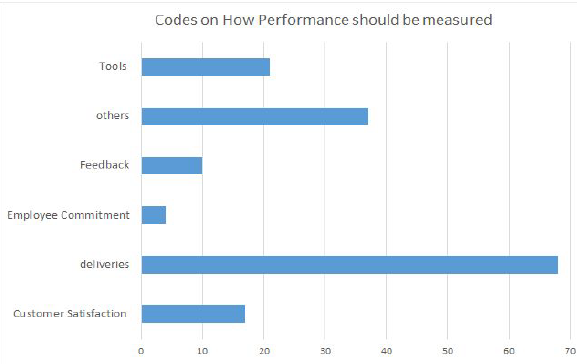
\includegraphics[width=15cm, height=8cm]{figure/auxiliary/fig513.PNG}
    \caption{How the performance should be measured in future?}
    \label{fig:5.13}
\end{figure}
   As mentioned before the responses were qualitative, hence it was coded by categorizing the similar responses. The respondents had different views on how their performance could be measured, for instance through feedback or end results of projects. The views had 5 major categories as explained below:\\

    \begin{enumerate}
    \item \textbf{Tools:} This category includes views on various tools that could be used to measure performance, like PI planning, KPIs or the PBP tool. They mentioned if the tools were used correctly, by setting right targets and deadlines they would be efficient.  \\
    \item \textbf{Feedback:} The respondents in this category believed that getting or giving feedback on their work would help them improve performance. These feedbacks could be from the managers or team members\\ 
    \item \textbf{Employee commitment:} People under this category feel that if the employees are well committed or satisfied with their work, the company is performing well. This could also be judged based on the workload on each employee and their health.\\
    \item \textbf{Deliveries:} As seen in the fig 5.13, most responses fall under this category. It includes responses which claimed that good performance is visible with good deliveries. These could be product delivered, quality, project deliverables, and meeting the goals set by teams or managers.\\
    \item \textbf{Customer Satisfaction:} This set of respondents believed that based on customer satisfaction, the performance of teams could be assessed.  It can either be internal or external customer.\\

\end{enumerate}
The last category in the graph is “others”, which has responses of people who were unsure how their performance could be measured.\\
    \item \textbf{“Your concluding views about present and future KPI”.}\\
    This question provided respondents a perfect opportunity to present their insights about the KPIs. The responses were subjective and based on observation the following views were majorly encountered. These were categorized into 3 groups as follows:\\
    
\begin{enumerate}
    \item First set of employees thought that KPIs were not a good tool, and they were not needed at all. Few comments such as “ KPIs are dull way of measuring performance”, “They do not reflect the work done, hence a bad tool” depicted that they were not needed at all. Though there were very few who mentioned this, their input is also important to understand why they thought so and what could be improved. This set of members also includes people who thought the KPIs were nowhere related to them and they were not the right way to summarize or measure their work.\\
    
    \item The Second set of employees believed that the present KPIs could be improved and suggestions on how they could be improved were given as follows:\\
    \begin{itemize}
    \item The KPIs needed better strategic breakdown\\
    \item KPIs lacked a sense of engagement\\
    \item Need to create buy in from employees \\
    \item The KPIs are too many in number. \\
    \item KPIs are not visible to the employees\\
    \item KPIs are a “Tool for Suboptimization” \\
    \item KPIs must meet the customer expectations\\
    \item KPIs needed more top management focus \\
    \item KPIs needed to reflect the quality of work \\

    \end{itemize}
    \item The last set of employees believed that KPIs were good tool and currently doing good. They had a positive view on the KPIs. This set had hardly few members, but had a positive view about the present KPIs.\\
\end{enumerate}

    \item The next 2 questions were simple. The intention was to know how the new organizational changes such as PE Next Gear and Agile transformation were perceived by employees. This data was important to know because the final analysis had to be made based on the importance of these issues. The respondents had to vote in levels 1-6. 1 being hindering my performance and 6 being improving my performance.\\
    \begin{figure}[H]
    \centering
    \captionsetup{justification=centering, margin=2cm}
    \vspace{1cm}
    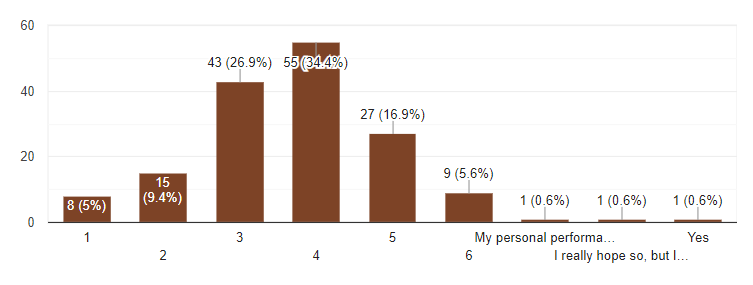
\includegraphics[width=14cm, height=6cm]{figure/auxiliary/fig514.PNG}
    \caption{How will PE next gear affect performance according to survey}
    \label{fig:5.14}
\end{figure}
    \begin{itemize}
        \item \textbf{PE Next gear:}\\
        As visible from the figure \ref{fig:5.14}, Approximately 57\% of employees leaned towards the second half of the spectrum. But still, one could easily notice that employees are not 100\% sure to choose the sides and are approximating their choice.\\
        \begin{figure}[H]
    \centering
    \captionsetup{justification=centering, margin=2cm}
    \vspace{1cm}
    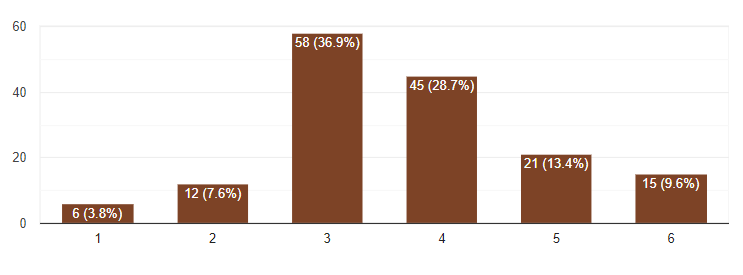
\includegraphics[width=14cm, height=6cm]{figure/auxiliary/fig515.PNG}
    \caption{How will agile transformation affect performance according to survey}
    \label{fig:5.15}
\end{figure}
        \item \textbf{Agile Transformation:}\\
        
        As visible from the fig 5.15, Approximately 52\% of employees leaned towards the second half of the spectrum. But still, one could easily notice that almost other half of employees feel agile way of working will not be conducive. Also, the highest response was level 3, indicating it would not be suitable for their line of work.\\

    \end{itemize}

\end{enumerate}
